\documentclass[]{manual}

\title{Fabry-Perot Interferometers}
\date{\today}
\course{Physics 325}

\begin{document}
    \maketitle
    \thispagestyle{firstpage}

    %%%

    \section{Motivation}

    The Fabry-Perot interferometer is a refinement of the Michelson interferometer.
    Instead of splitting a beam of light and interfering it with its other half a single time, a Fabry-Perot interferometer interferes the same beam of light with itself tens, hundreds, or even thousands of times.
    This dramatically increases the wavelength resolution of the interferometer, so much so that it can be used to look at the fine structure of individual transitions.
    In this lab we will look yet again at the sodium lamp, but this time we will be able to observe an interesting plasma phenomenon and distinguish the two orange emission lines in our scan.
    We will also look at the complicated structure of the green emission line in a low-pressure mercury lamp.

    \section{Background}

    A simple Fabry-Perot interferometer is constructed from two plane-parallel mirrors, which form an \emph{optical cavity}.
    When a beam of light is incident on the device it is partially transmitted into the cavity between the mirrors.
    This transmitted beam reflects back and forth between the mirrors many times (depending on the reflectivity of the mirrors), producing a transmitted ray from the far mirror each time.
    This geometry is shown in Figure~\ref{fig:fabry-perot-geometry}.
    
    When these beams are recombined on a screen using a focusing lens, we see a fringe pattern resulting from constructive interference between successively transmitted rays.
    In this sense the fringe pattern is very similar to the Michelson interferometer's fringe pattern.
    In the Fabry-Perot interferometer we see a bright fringe when the round-trip optical path length in the cavity is an integer multiple of the wavelength:
    \begin{align}  \label{eqn:fabry-perot-fringes}
        2nd \cos{\theta} = m \lambda,
    \end{align}
    where $n$ is the index of refraction of the medium filling the cavity, $d$ is the length of the cavity, $\theta$ is the angle to the fringe from the center of the pattern, and $m$ is an integer.

    If the fringes occur at the same angles as in the Michelson interferometer, why does the Fabry-Perot interferometer have better resolution?
    The key is that the Fabry-Perot interferometer interferes many beams instead of just two.
    If we have, say, ten reflections and $2nd \cos{\theta}$ is just barely larger than an integer number of wavelengths, $10 \times 2nd \cos{\theta}$ will be large because of the factor of 10.
    Therefore there will be a large path difference between the first reflection and the last reflection.
    This amplification of the path difference makes the constructive interference occur over a smaller value of $2nd \cos{\theta}$ than in a Michelson interferometer.
    A Fabry-Perot cavity made with modern dielectric mirrors ($R > 99.99\%$) could have thousands or even hundreds of thousands of reflections, giving extremely narrow fringes.

    \begin{figure}
        \centering
    
        \begin{tikzpicture}[thick, scale=2]
            \draw[pattern = north west lines] (-.1,0) rectangle (0, 3);
            \draw[pattern = north west lines] (1.5,0) rectangle (1.6, 3);
            \draw[dashed, |<->|] (0,-.1) -- (1.5,-.1) node[midway, below] {$d$};
            \node at (.75, 2.5) {$n$};
            \node[font=\footnotesize] at (.75, 3.1) {Fabry-Perot Cavity};

            % y = x tan(theta) = 1.5 * tan(10 deg) = .2645
            % r = x / cos(theta) = 1.5 / cos(10 deg) = 1.523

            \draw (0, 0.2) -- ++ (10:-1.2) node[below, font=\footnotesize] {Incident Ray};

            \draw[midarrow={latex}] (0, 0.2) -- ++(10:1.523);
            \draw[midarrow={latex}] (1.5, .4645) -- ++(170:1.523);
            \draw[neararrow={latex}] (1.5, .4645) -- ++(10:2) -- (5, 1.5225 + .6171);

            \draw[midarrow={latex}] (0, .729) -- ++(10:1.523);
            \draw[midarrow={latex}] (1.5, .9935) -- ++(170:1.523);
            \draw[neararrow={latex}] (1.5, .9935) -- ++(10:2) -- (5, 1.5225 + .6171);

            \draw[midarrow={latex}] (0, 1.258) -- ++(10:1.523);
            \draw[midarrow={latex}] (1.5, 1.5225) -- ++(170:1.523);
            \draw[neararrow={latex}] (1.5, 1.5225) -- ++(10:2) -- (5, 1.5225 + .6171);

            \draw[midarrow={latex}] (0, 1.787) -- ++(10:1.523);
            \draw[midarrow={latex}, path fading = west] (1.5, 2.0505) -- ++(170:1.523);
            \draw[neararrow={latex}, path fading = east] (1.5, 2.0505) -- ++(10:2) -- (5, 1.5225 + .6171);

            \pgfmathsetmacro{\lensRadius}{10}
            \pgfmathsetmacro{\lensHeight}{1.4}
            \pgfmathsetmacro{\startAngle}{asin(\lensHeight/\lensRadius)}

            % x = r * cos(theta) = 2 / cos(10 deg) = 1.97

            \draw[thin, gray] (1.5 + 1.97, 1.85 + \lensHeight) -- (1.5 + 1.97, 1.85 - \lensHeight) node[below, font=\footnotesize, black] {Lens};
            \draw (1.5 + 1.97, 1.85 + \lensHeight)
            arc[thick, start angle=180-\startAngle,delta angle=2*\startAngle,radius=\lensRadius]
            arc[thick, start angle=-\startAngle,delta angle=2*\startAngle,radius=\lensRadius]
            -- cycle; % to get a better line end
            

            \draw (5, 0) -- (5, 3) node[above, font=\footnotesize] {Screen};

            \draw[dashed] (0, .2) -- (-1.2, .2);
            \draw [<->, domain=180:190] plot ({cos(\x)}, {.2 + sin(\x)});
            \node[left] at (-1.1, .09) {$\theta$};

            \draw[dashed] (1.5 + 1.97, 1.85) -- (5, 1.85);
            \draw [<->, domain=0:12] plot ({1.5 + 1.97 + .9 * cos(\x)}, {1.85 + .9 * sin(\x)});
            \node[left] at (1.5 + 1.97 + .93, 1.92) {$\theta$};
        \end{tikzpicture}

        \caption{The geometry of a Fabry-Perot cavity.}
        
        \label{fig:fabry-perot-geometry}
    \end{figure}

    The green light from a \emph{low-pressure mercury lamp} ($\lambda \approx \SI{546}{\nano\meter}$) is particularly interesting to look at with the Fabry-Perot interferometer because it reveals that mercury on Earth typically has several isotopes of slightly different masses mixed in.
    Each isotope's emission lines are at slightly different wavelengths.
    We will also have enough resolution to see the fine structure of the atomic transitions, caused by relativistic corrections and the coupling of the electron's spin and angular momentum.
    A sample mercury spectrum made with a grating spectrometer is shown in Figure~\ref{fig:low-pressure-mercury-spectrum}.

    \begin{figure}[H]
        \centering
        
        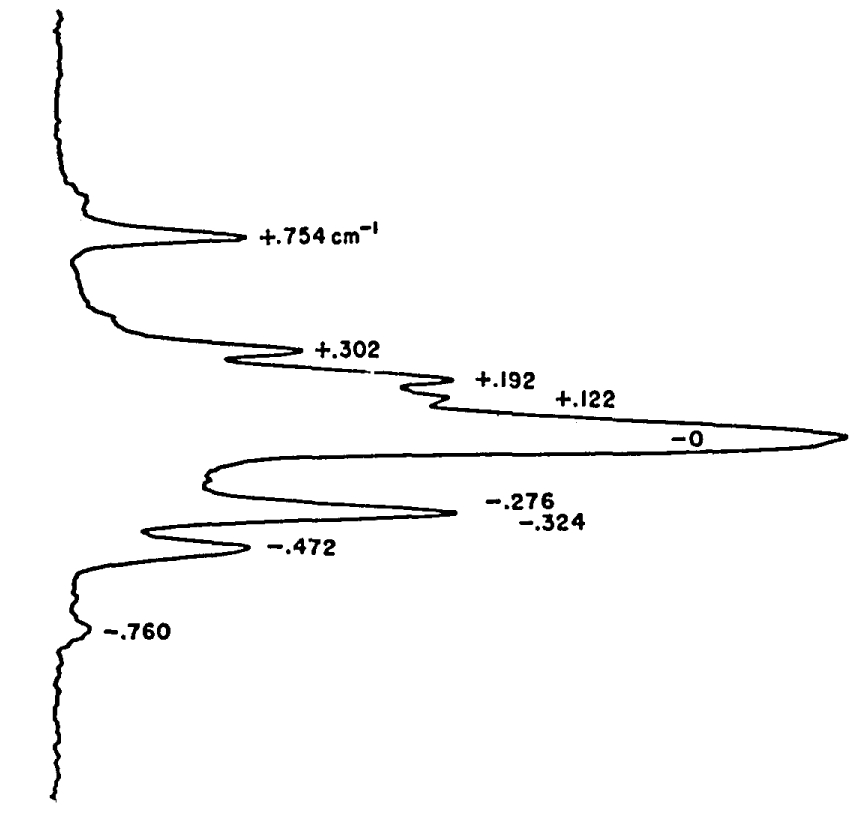
\includegraphics[width = .5\textwidth, angle = 90]{figs/hg_spectrum}
        
        \caption[Low-Pressure Mercury Spectrum]{W. Fastie, H. Crosswhite, and P. Gloersen, "Vacuum Ebert Grating Spectrometer," J. Opt. Soc. Am. 48, 106-111 (1958).}
        
        \label{fig:low-pressure-mercury-spectrum}
    \end{figure}

    \section{Equipment}

    In this lab you will use a pre-built Fabry-Perot cavity ($d=\SI{3}{\milli\meter}$) as your interferometer.
    The cavity is attached by alignment screws to a solid plate so that the cavity can be aimed at a photomultiplier tube.
    The Fabry-Perot cavity is fragile, so be careful when handling it.
    The cavity is attached to a source of compressed nitrogen gas which can be used to change the index of refraction between the plates (the index of refraction will increase as more nitrogen is added). 
    A manometer is built-in to the nitrogen supply to measure the pressure relative to the surrounding atmosphere.

    The photomultiplier tube uses high-voltage plates to convert a small flux of photoelectrons from the interferometer into a measurable current.
    The photomultiplier requires a negative voltage to operate.
    \emph{Do not exceed 600 volts on the photomultiplier!}

    \newpage

    \section{Procedure}

    \subsection{Aligning the Interferometer}
    Aligning the Fabry-Perot interferometer is significantly simpler than the Michelson interferometer because the Fabry-Perot cavity has been pre-assembled.
    However, you do need to make sure it is pointing in the right direction and that the output is focused onto the detector.

    \begin{enumerate}
        \item Get as much light from the sodium lamp going through the cavity as possible.
        \item Hold up a piece of paper on the far side of the focusing lens and find the focal plane (the distance from the lens where the bright fringes are sharpest).
        \item Move the photomultiplier so that the entrance iris is in the focal plane (the focal length of the lens is around $\SI{50}{\centi\meter}$).
        \item Tilt and tip the cavity using the knobs on the cavity assembly to send the center of the fringe pattern through the center of the iris. Use a piece of paper held near the photomultiplier iris to determine where the center of the pattern is.
        \item Close both irises (focusing lens and photomultiplier) until just a small amount of light is passing through them.
    \end{enumerate}

    We perform these steps to ensure maximum sensitivity.
    If the photomultiplier iris is not in the focal plane the recombining transmitted rays will have their phases shifted by the lens and the sharp fringe pattern will tend to spread out.
    Aligning the center of the fringe pattern ensures we get maximum signal.
    Closing down both irises minimizes any possible distortion in the alignment (since we are only using light from a very small region of the Fabry-Perot cavity).

    \subsection{Measuring the Index of Refraction of Nitrogen Gas}

    \subsubsection{Pressure Scanning \hfill (2 pts.)}
    Since the index of refraction of the material filling the Fabry-Perot cavity changes the optical path length in the cavity, we should be able to use it to measure the index of refraction of a gas.
    Perform a ``pressure scan'' by slowly filling the cavity with extra nitrogen gas. As you do this the angle of a given fringe will shift.
    As they pass through $\theta = 0$ the photomultiplier will detect them and you will see a signal on the electrometer.
    Therefore, you are mapping out a pressure vs. intensity curve (both indirectly, via the manometer and electrometer respectively).

    The first noteworthy aspect of this spectrum is that the fringes appear to come in pairs.
    We are seeing the two different wavelengths in the sodium emission line producing their own fringe patterns.
    In the Michelson interferometer these patterns blurred together, but in the Fabry-Perot interferometer they are quite distinct.

    The second noteworthy aspect is the \emph{self-reversal} of each line.
    The center of the plasma in the sodium lamp is much hotter than the outer edges.
    The emission line from the center region is thermally broadened and very bright compared to emission from the edges.
    In fact, the sodium plasma is cool enough at the edges that in that region it actually absorbs more photons than it emits.
    Since the transition is narrower at the edges, we see an absorption feature in the center of the broad emission line produced at the center of the plasma.

    Put a printout of a pressure scan from atmospheric pressure to atmospheric pressure plus $\SI{1000}{\torr}$ of nitrogen gas with both of these effects clearly labeled in your lab notebook.

    \subsubsection{Index of Refraction Measurement \hfill (4 pts.)}
    To measure the index of refraction using your pressure spectrum, note that the index of refraction of a low-density gas goes like
    \begin{align} \label{eqn:index-of-refraction}
        n \approx 1 + \alpha \, \frac{N}{V} = 1 + \alpha \, \frac{P}{RT},
    \end{align}
    where $N/V$ is the number density of the gas, $\alpha$ is a constant, $P$ is the pressure of the gas, $T$ is the temperature of the gas, and $R$ is the ideal gas constant. We could use this equation to determine the index of refraction of nitrogen gas at standard temperature and pressure ($P = \SI{760}{\torr}$, $T = \SI{273.15}{\kelvin}$) if we can determine $\alpha$.

    Figure out a way to measure $\alpha$, measure it, and compute the index of refraction of nitrogen gas at standard temperature and pressure, $n_{\mathrm{STP}}$.
    The accepted value is 1.000298 - how close did you get?
    Keep in mind that you can't include the overall 1 in your error analysis - we only care about the difference of the index of refraction from 1, because that's the index of refraction of vacuum.

    \subsubsection{The Fine and Isotopic Structure of Mercury \hfill [2 pts.]}
    Swap out the sodium lamp for the low-pressure mercury lamp.
    Perform the same kind of pressure scan as before.
    If you do not see at least six or seven distinguishable peaks, you will need to go back to the sodium lamp and ensure that you have the setup very well aligned.
    Print out your pressure scan and note the emission lines that you can distinguish.

    \newpage
    \section{Prelab Questions}
    \setcounter{subsection}{0}
    
    \subsection{Fringe Movements \hfill (1 pt.)}
    
    Suppose we have the interferometer showing a bullseye interference pattern at room pressure.
    As the pressure in the cavity is increased, does a given fringe $m$ move in (to smaller $\theta$) or out (to larger $\theta$)?
    
    \vspace{\stretch{1}}
    
    \subsection{Finessing Your Measurements \hfill (1 pt.)}
    From Equation~\ref{fig:low-pressure-mercury-spectrum} we can deduce that the green emission line in low-pressure mercury is approximately \SI{5}{\giga\hertz} wide.
    The \emph{free spectral range} (frequency distance between adjacent transmission peaks) of a $d=\SI{3}{\milli\meter}$ Fabry-Perot cavity is $\mathrm{FSR} = c / 2d \approx \SI{50}{\giga\hertz}$.
    The \emph{finesse} of the cavity is the ratio between the free spectral range and the width of the cavity transmission line, $\mathcal{F} = \Delta \nu / \mathrm{FSR}$, but is also approximately equal to the number of round-trips each photon will go through in the cavity.
    
    Estimate (to within an order of magnitude) the minimum finesse that the Fabry-Perot interferometer used in this experiment needs to achieve to be able to resolve the fine structure of the green emission line in low-pressure mercury.
    
    \vspace{\stretch{1}}

\end{document}
